\usetikzlibrary{arrows}
\usetikzlibrary{positioning}

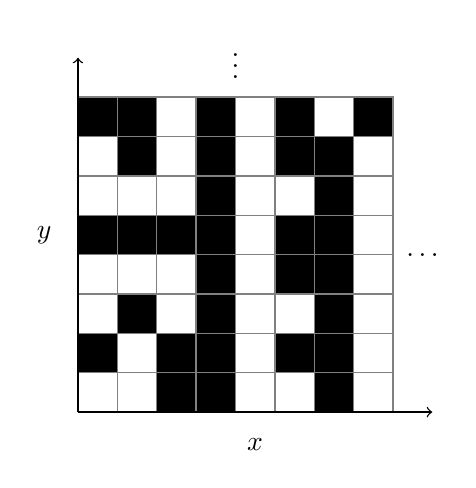
\begin{tikzpicture}[line width =0.5pt, scale=0.5]

\draw[gray] (0,0) grid (8,8);
\foreach \x/\y in {0/1, 0/4, 0/7, 1/2, 1/4, 1/6, 1/7, 2/0, 2/1, 2/4, 3/0, 3/1, 3/2, 3/3, 3/4, 3/5, 3/6, 3/7, 5/1, 5/3, 5/4, 5/6, 5/7, 6/0, 6/1, 6/2, 6/3, 6/4, 6/5, 6/6, 7/7}
    \filldraw[fill=black, draw=gray] (\x,\y) rectangle ++(1,1);
\draw[->] (0,0) -- (9,0) node[midway, below=6pt]{$x$};
\draw[->] (0,0) -- (0,9) node[midway, left=6pt]{$y$};
\node[] at (4,9){$\vdots$};
\node[] at (8.75,4){$\dots$};
\end{tikzpicture}